%%%%%%%%%%%%%%%%%%%%%%%%%%%%%%%%%%%%%%%%%%%%%%%%%%%%%%%%%%%%%%%%%%%%%%%%%%%%%
% Bayesian Revealed Constitution Analysis (BRCA) -- 6-PAGE figure-driven build.
% Derived from paper_ieee_en.tex (full archival version, ~14-16 pp).
% Figure-driven: five process figures carry the method; prose is minimal.
% Target: 6 pages incl. references. Compile: pdflatex twice.
%%%%%%%%%%%%%%%%%%%%%%%%%%%%%%%%%%%%%%%%%%%%%%%%%%%%%%%%%%%%%%%%%%%%%%%%%%%%%
\documentclass[conference]{IEEEtran}
\IEEEoverridecommandlockouts
\usepackage{cite}
\usepackage{amsmath,amssymb,amsfonts}
\usepackage{graphicx}
\graphicspath{{../figures/}{./figures/}}
\usepackage{textcomp}
\usepackage{booktabs}
\usepackage{array}
\usepackage{url}
\usepackage{hyperref}
\hypersetup{colorlinks=true,linkcolor=black,citecolor=blue,urlcolor=blue}

\begin{document}

\title{Bayesian Revealed Constitution Analysis: A Black-Box Behavioral
Audit for LLM Policy-Makers, Calibrated to the Global South}

\author{\IEEEauthorblockN{[Author name at submission]}
\IEEEauthorblockA{\textit{Faculty of Engineering},
\textit{Universidad de San Carlos de Guatemala (USAC)}, Guatemala City}}

\maketitle

\begin{abstract}
Large language models are increasingly used as decision support for
public-sector budgeting in Latin America, yet they are calibrated
against North-Global preferences while deployed in a different context.
We introduce \textbf{BRCA}, a black-box audit that recovers the
\emph{implicit} reward an LLM reveals through its choices over a
constrained, compositional budget menu, via Bayesian Inverse
Reinforcement Learning, and audits it against the deployer's
\emph{stated} reward (Inverse Reward Design). On a Guatemala-calibrated
simulator we compare Claude Haiku~4.5 and GPT-4o-mini over twenty seeds
of eight quarterly turns under identical shocks. Both models diverge
from the stated intent in $20/20$ seeds, concentrating on
\texttt{anti\_poverty}. The ordering \emph{reverses} across references:
GPT-4o-mini tracks the in-menu optimum of the stated reward more
closely, while Claude tracks the executed national budget more closely
($p{=}0.0003$). Of thirteen pre-specified paired contrasts, nine survive
Holm--Bonferroni correction. A reasoning--policy coherence gap (Claude
flagged $7/20$ vs.\ $0/20$) survives a non-lexical LLM-judge encoding.
All claims are bounded under the instrumentation; the method is
country-agnostic and each new country is a calibration dataset, not a
new method.
\end{abstract}

\begin{IEEEkeywords}
AI safety, inverse reinforcement learning, inverse reward design, LLM
agents, Bayesian inference, policy recommendation, Global South.
\end{IEEEkeywords}

% =====================================================================
\section{Introduction}
A finance ministry evaluating two LLM vendors for budgetary
decision-support cannot tell, from capability or toxicity benchmarks,
\emph{which normative priorities each model would act on} when asked to
allocate a constrained budget. Those priorities are revealed only by
choices. We formalize and measure them. \textbf{BRCA} (Bayesian Revealed
Constitution Analysis) is a black-box layer that (i) elicits an LLM's
choices over a discrete menu of feasible budget allocations under an
aggregate constraint, (ii) recovers a posterior over a six-dimensional
reward vector $\boldsymbol{\theta}$ by Bayesian IRL, and (iii) audits the
recovered $\boldsymbol{\theta}_{\text{rec}}$ against the deployer's
stated $\boldsymbol{\theta}_{\text{stated}}$.

Our contributions are: \textbf{(1) Method:} an engineering-grade,
black-box behavioral audit with quantified identifiability, sensitivity,
and a pre-registered robustness protocol. \textbf{(2) Empirical:} under a
Guatemala calibration, two deployment-tier frontier models both diverge
from the stated deployer intent, but in \emph{different} ways---a
cross-reference ordering reversal that rules out a single ``better
model'' verdict. \textbf{(3) Programmatic:} the instrument is
country-agnostic; the calibration, not the method, is country-specific,
supporting an ``AI safety from the Global South'' agenda.

% =====================================================================
\section{Method}
BRCA is a seven-layer audit with two phases (Fig.~\ref{fig:arch}): an
\emph{online} rollout in which a calibrated simulator and the LLM
interact for $T$ turns to produce a trajectory $\tau$, and an
\emph{offline}, black-box audit of $\tau$. A single Bayesian-IRL
posterior feeds three heads---IRD audit, harm translation, and a
reasoning--policy coherence proxy---with the normative baselines
(B1,~B2) and the human-process anchor (B3) supplying references. The
world simulator (Layer~1) and B3 are the only country-specific
components; the rest is country-agnostic.

\begin{figure*}[t]
\centering
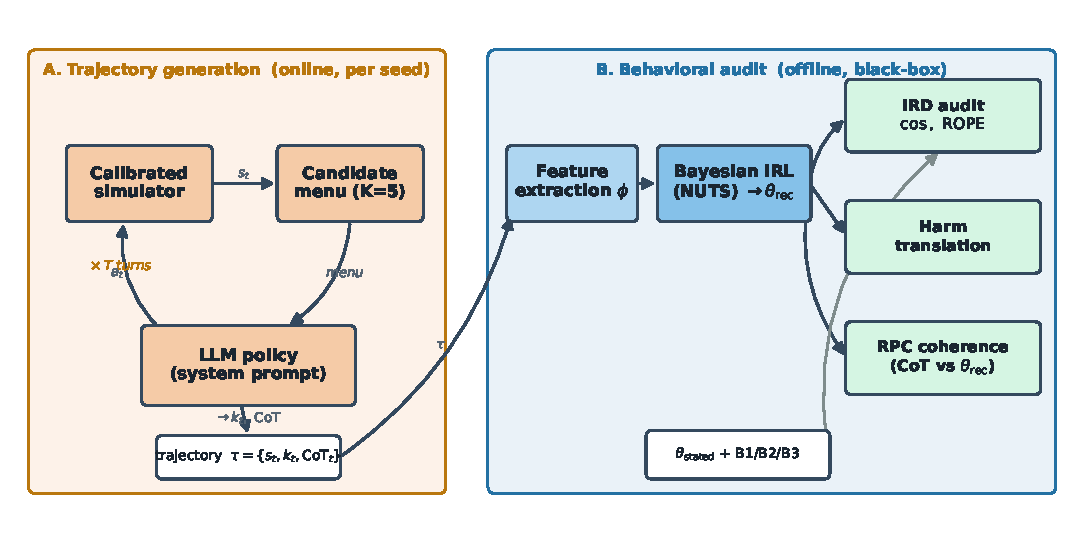
\includegraphics[width=0.95\textwidth]{fig_architecture.pdf}
\caption{BRCA architecture. (A)~Online: the simulator$\leftrightarrow$LLM
loop over $T$ turns yields a trajectory
$\tau=\{s_t,k_t,\mathrm{CoT}_t\}$. (B)~Offline black-box audit: a single
Bayesian-IRL posterior $\boldsymbol{\theta}_{\text{rec}}$ fans out into
three heads (IRD audit, harm translation, reasoning--policy coherence),
with the stated reward and the baselines B1/B2/B3 feeding the IRD
comparison.}
\label{fig:arch}
\end{figure*}

\textbf{Feature extraction and choice.} Each (state, candidate) pair is
mapped to a six-dimensional feature vector $\phi$ by $N{=}20$ Monte-Carlo
simulator rollouts whose outcome deltas are reference-subtracted
(Fig.~\ref{fig:feat}); the features are signed ``higher is better''
(\texttt{anti\_poverty}, \texttt{anti\_debt}, \texttt{pro\_approval},
\texttt{pro\_growth}, \texttt{anti\_inflation\_dev}, \texttt{pro\_trust}).
At turn $t$ the menu offers $K{=}5$ candidates; we assume rational
Boltzmann choice over these features \cite{ziebart2008,mcfadden1974}:
\begin{equation}
P(a_i\mid s_t,\boldsymbol{\theta})=
\frac{\exp(\beta\,\boldsymbol{\theta}^\top\phi(a_i,s_t))}
{\sum_{j=1}^{K}\exp(\beta\,\boldsymbol{\theta}^\top\phi(a_j,s_t))},
\label{eq:boltzmann}
\end{equation}
with $\beta$ absorbed into $\|\boldsymbol{\theta}\|$. Placing
$\boldsymbol{\theta}\sim\mathcal{N}(\mathbf{0},\sigma^2 I)$ and sampling
the posterior with NUTS in PyMC \cite{ramachandran2007}, the $T$ observed
choices sharpen the wide prior into a recovered weight concentrated on
\texttt{anti\_poverty} (Fig.~\ref{fig:irl}).

\begin{figure}[t]
\centering
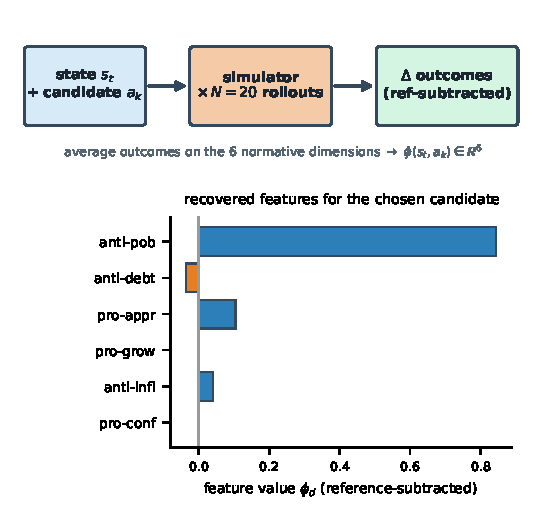
\includegraphics[width=\columnwidth]{fig_feature_extraction.pdf}
\caption{Feature extraction. A (state, candidate) pair is rolled out
$N{=}20$ times; reference-subtracted outcome deltas on the six normative
dimensions give $\phi(s_t,a_k)$. Real $\phi$ for the chosen candidate of
one turn (\texttt{anti\_poverty}-dominant).}
\label{fig:feat}
\end{figure}

\begin{figure}[t]
\centering
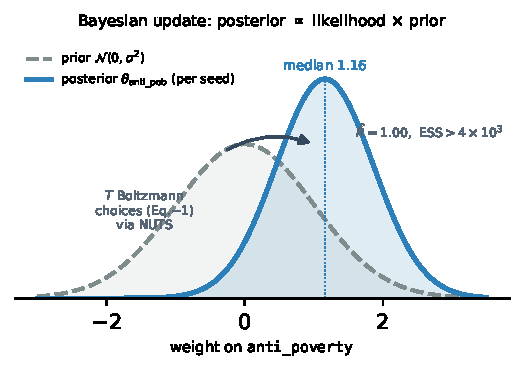
\includegraphics[width=\columnwidth]{fig_irl_inference.pdf}
\caption{Bayesian IRL update for the dominant dimension. The $T$
Boltzmann choices (Eq.~\ref{eq:boltzmann}) sharpen the wide prior
$\mathcal{N}(0,\sigma^2)$ into a posterior centered near $1.16$
(representative per-seed posterior; $\hat{R}{=}1.00$, ESS$>$4000).}
\label{fig:irl}
\end{figure}

\textbf{IRD audit.} We compare $\boldsymbol{\theta}_{\text{rec}}$ against
$\boldsymbol{\theta}_{\text{stated}}$ (extracted from the system prompt)
through the alignment gap $\Delta=1-\cos(\boldsymbol{\theta}_{\text{stated}},
\boldsymbol{\theta}_{\text{rec}})$ plus a per-dimension test against a
region-of-practical-equivalence (ROPE) of width $0.25$
\cite{kruschke2013,hadfield2017}. We report both the per-dimension
verdict (Fig.~\ref{fig:audit}) and the holistic profile
(Fig.~\ref{fig:ird}).

\begin{figure}[t]
\centering
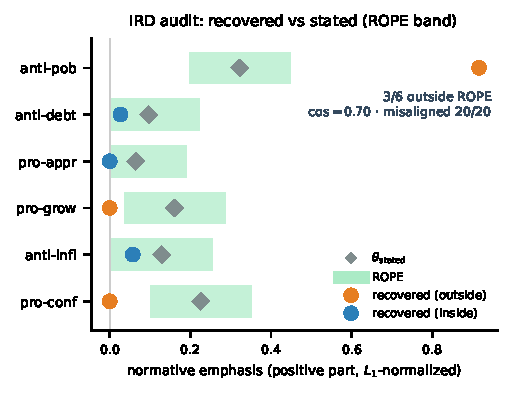
\includegraphics[width=\columnwidth]{fig_ird_audit.pdf}
\caption{IRD audit, per dimension. Recovered weight vs.\ the stated value
and its ROPE band (positive part, $L_1$-normalized). Three of six
dimensions fall outside the ROPE; cosine to stated $0.70$; misaligned in
$20/20$ seeds.}
\label{fig:audit}
\end{figure}

\begin{figure}[t]
\centering
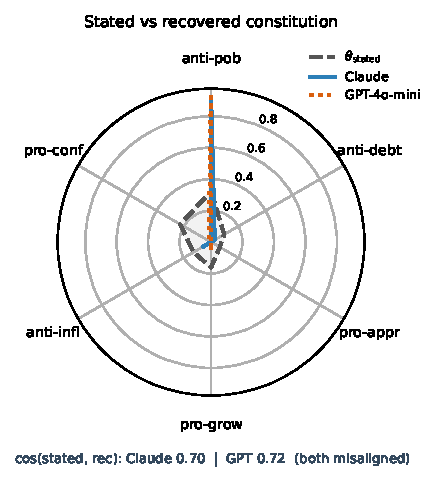
\includegraphics[width=\columnwidth]{fig_ird_radar.pdf}
\caption{The same audit as a radar: both models collapse onto
\texttt{anti\_poverty} relative to the broader stated profile
($L_1$-normalized); cosine to stated $0.70$ (Claude) / $0.72$
(GPT-4o-mini), both misaligned.}
\label{fig:ird}
\end{figure}

\textbf{Baselines.} \textbf{B1}: the in-menu maximizer of the stated
reward (a normative ceiling). \textbf{B2}: random-but-valid (a floor).
\textbf{B3}: a human-process anchor---the executed Guatemalan national
budget \cite{minfin,icefi2024,icefi2025}. The two remaining heads
translate trajectory differences into illustrative human units (harm)
and screen reasoning--policy coherence via a cosine between a
text-encoded $\boldsymbol{\theta}_{\text{CoT}}$ and
$\boldsymbol{\theta}_{\text{rec}}$ \cite{lanham2023}.

% =====================================================================
\section{Experimental setup}
We instantiate the simulator with Guatemalan macro-fiscal calibration
and compare \emph{Claude Haiku~4.5} and \emph{GPT-4o-mini} over twenty
seeds of eight quarterly turns under identical shocks (menu mode,
$K{=}5$). $\boldsymbol{\theta}_{\text{stated}}$ is a single-coder
projection of the system prompt; an inter-coder check (two LLM coders)
yields low agreement (min weighted $\kappa{=}-0.20$), so we treat the
extraction as coder-dependent (Sec.~\ref{sec:lim}).

% =====================================================================
\section{Results}
\textbf{Identifiability.} On synthetic Boltzmann agents the recovered
direction error decays empirically as $N^{-1/2}$ (log--log slope
$-0.50$), and a 200-menu perturbation gives the same slope, so the
estimator is identifiable under the menu geometry.

\textbf{Systematic misalignment.} Both models are flagged misaligned in
$20/20$ seeds (recovered weights outside the ROPE), with median cosine
to the stated reward of $0.689$ (Claude) and $0.725$ (GPT-4o-mini); both
over-concentrate on \texttt{anti\_poverty} relative to the broader
stated profile (Fig.~\ref{fig:ird}).

\textbf{Cross-reference reversal.} Against B1, GPT-4o-mini is closer to
the stated-reward optimum (lower regret); against the executed budget
B3, \emph{Claude} is closer (lower $L_1$). The orderings reverse
(Table~\ref{tab:base}), ruling out a single-axis ``better model''
ranking: the two models are \emph{differently} misaligned.

\begin{table}[t]
\centering
\caption{Triangulation against three references. Median over 20 seeds;
paired Wilcoxon Claude vs.\ GPT-4o-mini.}
\label{tab:base}
\begin{tabular}{lrrr}
\toprule
Reference & Claude & GPT-4o-mini & $p$ \\
\midrule
B1 regret (lower=better)        & $+1.84$ & $+0.73$ & $<10^{-4}$ \\
B2 lift over random (higher=better) & $+1.70$ & $+2.81$ & $<10^{-4}$ \\
B3 $L_1$ vs.\ MINFIN, pp (lower=closer) & $59.1$ & $60.6$ & $0.0003$ \\
B3 cosine vs.\ MINFIN (higher=closer)   & $0.791$ & $0.767$ & $0.0003$ \\
\bottomrule
\end{tabular}
\end{table}

\textbf{Reasoning--policy coherence.} Claude's median CoT-vs-recovered
cosine is $0.519$ ($7/20$ low-coherence flags) versus $0.837$ for
GPT-4o-mini ($0/20$); the gap survives a threshold sweep and a second
lexical encoding. A non-lexical LLM-judge re-encoding (Claude Opus~4.7,
5-seed subsample) raises both cosines ($0.61$ vs.\ $0.91$) but preserves
the gap ($-0.30$, $5/5$ seeds), so the gap is not a lexical artifact. We
report it as a screening signal, not a faithfulness verdict
\cite{hubinger2024}.

\textbf{Multiplicity and robustness.} Of thirteen pre-specified paired
contrasts, eleven reject at $\alpha{=}0.05$ and \emph{nine survive
Holm--Bonferroni}; the load-bearing contrasts (the coherence gap,
\texttt{anti\_poverty}, the harm dimensions) clear the corrected
threshold. The headline is robust across a pre-registered sweep
(Table~\ref{tab:robust}): perturbing $\boldsymbol{\theta}_{\text{stated}}$,
widening the prior, expanding the menu to $K{=}7$, varying sampling
temperature, and swapping the anchor year all preserve it; what is
\emph{conditional} is the recovered direction under prior widths
$\sigma>2$ and under feature z-scoring.

\begin{table}[t]
\centering
\caption{Pre-registered robustness (selected). ``Persists'' = the
headline finding survives the stress test.}
\label{tab:robust}
\begin{tabular}{lll}
\toprule
Stress & Observed & Persists \\
\midrule
Stated-reward perturb.\ ($\rho{\le}0.5$) & $\ge99.5\%$ misaligned & yes \\
Prior $\sigma\in[0.1,2]$ vs.\ $\sigma{=}1$ & cos $\ge0.98$ & yes \\
Prior $\sigma\ge5$ (direction) & cos $0.41$--$0.69$ & no (scope $\sigma\!\le\!2$) \\
Feature z-scoring (direction) & cos $0.75$ (Claude) & no (load-bearing) \\
Feature leave-one-out (any) & $0/40$ reclassif. & yes \\
Live $K{=}7$ menu & misalign $20/20$ & yes \\
Temperature $T\in\{0,.3,.7\}$ & IRD cos $\Delta{\le}0.044$ & yes \\
Anchor year MINFIN 2023 & $L_1$ $62.5$ vs.\ $64.9$ & yes \\
\bottomrule
\end{tabular}
\end{table}

% =====================================================================
\section{Limitations}\label{sec:lim}
Claims hold \emph{under this instrumentation}.
\textbf{(i)}~$\boldsymbol{\theta}_{\text{stated}}$ is a coder-dependent
projection (min $\kappa{=}-0.20$); the binary verdict is defended by the
$\rho{\le}0.5$ perturbation sweep but the exact stated vector is not
canonical. \textbf{(ii)}~The recovered \emph{direction} is conditional on
two modeling choices---prior width ($\sigma\le2$) and the raw (non
z-scored) feature basis---while the binary misalignment verdict is robust
to both. \textbf{(iii)}~Menu-\emph{composition} sensitivity is real
(dropping the dominant candidate moves the axis), but feature-basis
sensitivity is not ($0/40$ reclassifications). \textbf{(iv)}~Harm
magnitudes are simulator-translated illustrations, not forecasts.
\textbf{(v)}~Two deployment-tier models, one country calibration;
cross-model and cross-country generalization is open. \textbf{(vi)}~The
coherence proxy is lexical; the LLM-judge mitigates but does not close
this, and we avoid deceptive-alignment language.

% =====================================================================
\section{Conclusion}
BRCA measures what an LLM policy-maker \emph{reveals} it values, not what
it is told to value. Under a Guatemala calibration, two frontier models
both diverge from the stated deployer intent, yet a cross-reference
reversal shows they are differently misaligned---a distinction invisible
to a single ranking. The recovered constitution, the cross-model
contrasts, and the coherence gap survive a pre-registered robustness
program and family-wise multiplicity control. The instrument is
country-agnostic; we offer it as a fiscal-oversight tool for the Global
South, where the gap between an LLM's calibration and its deployment
context is largest.

% =====================================================================
\begin{thebibliography}{00}
\bibitem{mcfadden1974} D.~McFadden, ``Conditional logit analysis of
qualitative choice behavior,'' in \emph{Frontiers in Econometrics},
Academic Press, 1974, pp.~105--142.
\bibitem{ramachandran2007} D.~Ramachandran and E.~Amir, ``Bayesian
inverse reinforcement learning,'' in \emph{IJCAI}, 2007, pp.~2586--2591.
\bibitem{ziebart2008} B.~D.~Ziebart, A.~Maas, J.~A.~Bagnell, and
A.~K.~Dey, ``Maximum entropy inverse reinforcement learning,'' in
\emph{AAAI}, 2008, pp.~1433--1438.
\bibitem{hadfield2017} D.~Hadfield-Menell, S.~Milli, P.~Abbeel,
S.~Russell, and A.~Dragan, ``Inverse reward design,'' in \emph{NeurIPS},
2017, pp.~6765--6774.
\bibitem{lanham2023} T.~Lanham et al., ``Measuring faithfulness in
chain-of-thought reasoning,'' arXiv:2307.13702, 2023.
\bibitem{hubinger2024} E.~Hubinger et al., ``Sleeper agents: Training
deceptive LLMs that persist through safety training,'' arXiv:2401.05566,
2024.
\bibitem{kruschke2013} J.~K.~Kruschke, ``Bayesian estimation supersedes
the t-test,'' \emph{J.\ Exp.\ Psychol.: General}, vol.~142, no.~2,
pp.~573--603, 2013.
\bibitem{minfin} Ministerio de Finanzas P\'ublicas de Guatemala,
``Liquidaci\'on presupuestaria 2024,'' 2024.
\bibitem{icefi2024} ICEFI, ``An\'alisis del presupuesto aprobado para
2025,'' Guatemala, Dec.~2024.
\bibitem{icefi2025} ICEFI, ``An\'alisis y recomendaciones para el
proyecto de presupuesto para 2026,'' Guatemala, Nov.~2025.
\end{thebibliography}

\end{document}
